\def\firstname{Tim}
\def\lastname{Dahmen}
\def\aufgabenblatt{2 and 3}

\documentclass{article}

\usepackage[a4paper, margin=2.5cm]{geometry}
\usepackage{graphicx}
\usepackage[ngerman]{babel} % automatische Silbentrennung
\usepackage[table]{xcolor}
\usepackage{tabularx,array,booktabs,makecell}
\usepackage{titlesec}
\usepackage{amsmath}

\usepackage{fancyhdr}
\pagestyle{fancy} 
\fancyhead[L]{Inpainting SS 2024}  

\fancypagestyle{page1}{
	\fancyhead[L]{\firstname \: \lastname}
	\fancyhead[C]{Inpainting SS 2024\\Aufgabenblatt \aufgabenblatt}
	\fancyhead[R]{ \\
\includegraphics[width=0.25\textwidth]{../common/hs_aalen_de.png}}

}
\setlength{\parindent}{0mm}
\setlength{\parskip}{2.5mm}

\titlespacing*{\section}{0mm}{4pt}{0pt}
\setlength{\headsep}{14mm}

\begin{document}
\thispagestyle{page1} 

\section{Natural Neighbor Interpolation}

In canvas, you will find a file pixelliste.csv. This text file contains one defined pixel value per line in the format x-position, y-position, r-value, g-value, b-value, each separated by a semicolon.

\subsection{Read in Pixel List (5 points)}

Complete the code in the file natural\_neighbor\_interpolation.py. 

\begin{enumerate}

\item[a)] Complete the unit tests (test\_read\_pixel\_cloud\_from\_csv).

\item[b)] Describe your test strategy: which cases do you test and why? What could happen when reading a file, which cases are worth testing?\\
Test if rows in csv add up with value in row 0. Test if every row has 5 values. Test if expected types match.

\end{enumerate}

I needed the following time to complete the task: 5min

\subsection{Create Neighborhood Relation (10 points)}

The pixels in the list are in random order. In order to interpolate, we first have to reconstruct the neighborhood relationships, i.e. we have to determine which pixel is next to which. This relationship is not unique - there are generally several solutions. We determine the neighborhood via a Delauney triangulation. This means that we build a Voronoi diagram and define two pixels as neighboring if their Voronoy cells touch. 

\begin{enumerate}

\item[a)] Familiarize yourself with the documentation of the scipy.spatial.Voronoi and scipy.spatial.Delauney package. The function create\_delauney\_triangulation demonstrates how to use the package. We do not bother to reprogramming the algorithm at this point. 

\item[b)] Research the algorithm to create a Voronoi diagram on your own. Describe the algorithm in your own words.

\item[c)] Bonus task: Think about properties of our points: we have pixel coordinates, some of which are missing. Can you think of properties of these points that we could possibly use to create a Voronoi diagram faster than the implementation in scipy.spatial? 

\item[d)] Bonus task: Argue which development environments (programming language, compiler, hardware) could be considered, and which of them would be expected to lead to fast or slow code.

\end{enumerate}

The Voronoi diagram and the associated Delauney triangulation look like this:

\begin{center}
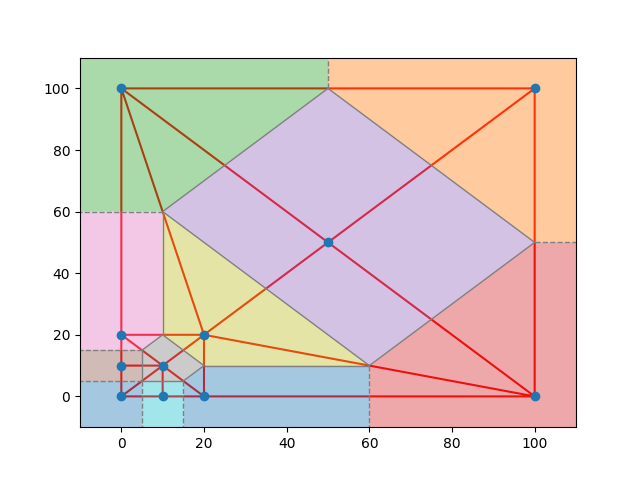
\includegraphics[width=0.5\textwidth]{source_code/example_delauney.png}
\end{center}

I needed the following time to complete the task:

\subsection{Barycentric coordinates (10 points)}

To be able to interpolate between three points of a triangle, we need a weighting between the points. An obvious possibility would be to weight each point with the reciprocal of the distance, normalized by the sum of the weights of all three vertices. 

\begin{enumerate}

\item[a)] Argue in your own words what the disadvantage of this method is.

\item[b)] Derive barycentric coordinates. The coordinates fulfill the following conditions: multiply each of the three vertices by its weight and add the coordinates to obtain the target point. This applies in the x-direction (condition 1) and y-direction (condition 2). In addition, the weights add up to 1 (normalizing condition). Derive a formula for
Barycentric coordinates by solving for $W_1$, $W_2$ and $W_3$.

Note: the derivation can easily be found on the Internet. Nevertheless, solve it yourself first.

\begin{align}
	P_x &= W_1 \cdot X_1 + W_2 \cdot X_2 + W_3 \cdot X_3 \\
	P_y &= W_1 \cdot Y_1 + W_2 \cdot Y_2 + W_3 \cdot Y_3 \\
	1 &= W_1 + W_2 + W_3
\end{align}

\item[c)] The function test\_compute\_barycentric\_coordinates already contains some test cases. Argue: are these test cases sufficient, or which test cases should be added? 

\item[d)] Add the test cases according to your argumentation from c). 

\item[e)] Complete the source code in the function compute\_barycentric\_coordinates. 

\end{enumerate}

I needed the following time to complete the task: 1h

\subsection{Interpolation of the pixel values (5 points)}

Now implement an interpolation method for pixel values: use the barycentric coordinates to interpolate color values. 

\begin{enumerate}

\item[a)] First add the test cases in test\_compute\_interpolated\_pixel\_value. Argue why you have added the test cases in exactly the same way. Not adding test cases if there are good reasons to do so is also a valid solution throughout the lecture. In this case, argue why you consider an addition to be unnecessary.

\item[b)] Now implement the function compute\_interpolated\_pixel\_value.

\end{enumerate}

I needed the following time to complete the task: 20min

\subsection{rasterization of triangles (20 points)}

Based on the function for interpolating pixel values, implement the complete natural neighbor interpolation.

\begin{enumerate}

\item[a)] You rasterize a triangle by first determining the axis aligned bounding box, i.e. the smallest and largest coordinate in the x and y directions. The triangle always lies within this box. As always: first add test cases or argue why this is not necessary.

\item[b)] Now iterate all pixels within the box. Use two nested loops. Calculate the interpolated color value for each pixel and save it in the array. If necessary, first add test cases. Then implement the function.

\item[c)] Not all pixels within the box are also within the triangle. This must be dealt with. A simple test of whether a point is inside a triangle uses barycentric coordinates: if one of the coordinates is negative, the point is outside. Build in an appropriate test. For example, the interpolation function could return None if the point is outside. You could also write a separate function (pixel\_inside\_trangle) and not even calculate the interpolated color values if the pixel is outside.

\begin{center}
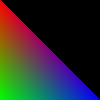
\includegraphics[width=0.25\textwidth]{source_code/interpolated.png}
\end{center}

\item[d)] You have been asked for help because a colleague's implementation has pixel errors. Maybe your implementation has the same problem? Speculate what could be causing the error and suggest a solution.

\begin{center}
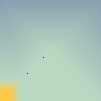
\includegraphics[width=0.25\textwidth]{source_code/example_pixel_error.png}
\end{center}

\end{enumerate}

I needed the following time to complete the task: 1h

\end{document}